\documentclass{beamer}
\usetheme{Berlin}
%\usecolortheme{dolphin}
\usepackage[utf8]{inputenc}
\usepackage[T1]{fontenc}
\usepackage[english]{babel}


\usepackage{csvsimple}
\usepackage{graphicx}
\graphicspath{ {./files/} } % Path relative to the main .tex file 
\newcommand{\fg}[2]{%
  \begin{center}
      \includegraphics[width = #1\textwidth]{#2}%
  \end{center}
}


\usepackage{verbatim}
%\usepackage{subfigure}
\usepackage{caption}
\usepackage{subcaption}





\title{Estimating Client Needs}

\subtitle{Business Case 2}

\author{T. Bucci, F. Cipriani, G. Corbo, D. Fabroni, M. Lucchini}

\institute{Politecnico di Milano}

\date{March 31, 2022}





\begin{document}

\frame{\titlepage}

\begin{frame}
    \frametitle{Table of Contents}
    \tableofcontents
\end{frame}

\section{Data and model exploration}
\begin{frame}[fragile]
    \frametitle{Goal: Recommendation System}
    We intend to estimate some investments needs for these customers using Data Science techniques.
    
    \vspace*{1cm}

    \textbf{Data:}\\

    Needs:\\
    {\tiny
    \begin{verbatim}
    	ID    Age    Gender    FamilyMembers    FinancialEducation    RiskPropensity
    	Income     Wealth    IncomeInvestment    AccumulationInvestment
    \end{verbatim}
    }

    Products:\\
    {\tiny
    \begin{verbatim}
    	IDProduct    Type    Risk
    \end{verbatim}
    }
    %\footnote{\texttt{https://www.kaggle.com/uciml/biomechanical-features-of-orthopedic-patients?select=column_3C_weka.csv}}
\end{frame}

\begin{frame}
	\frametitle{No significant sex difference}
	\begin{figure}
	   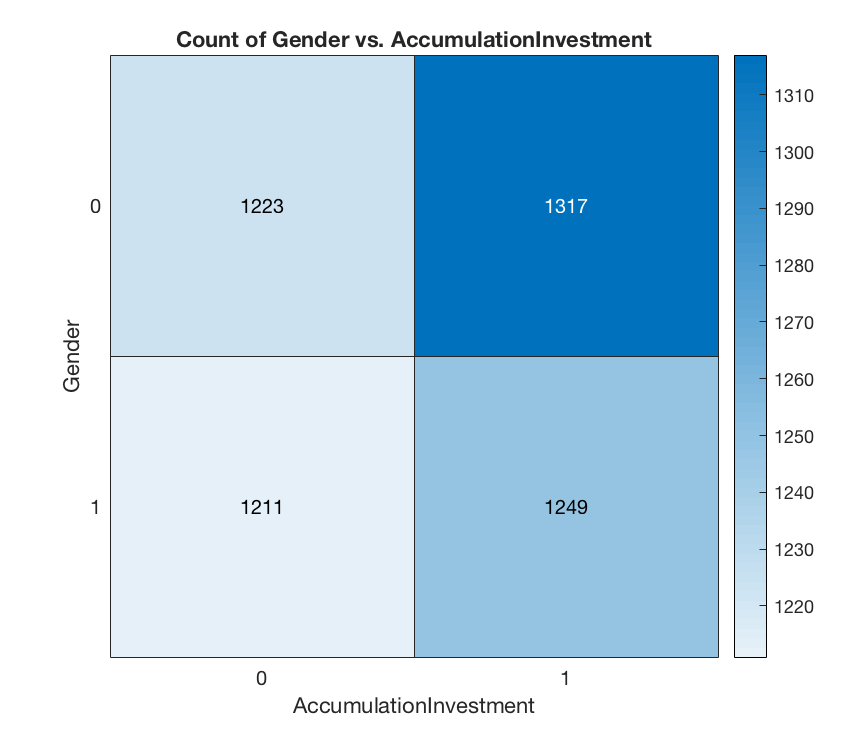
\includegraphics[width=0.48\textwidth]{hm2}
	   \hfill
	   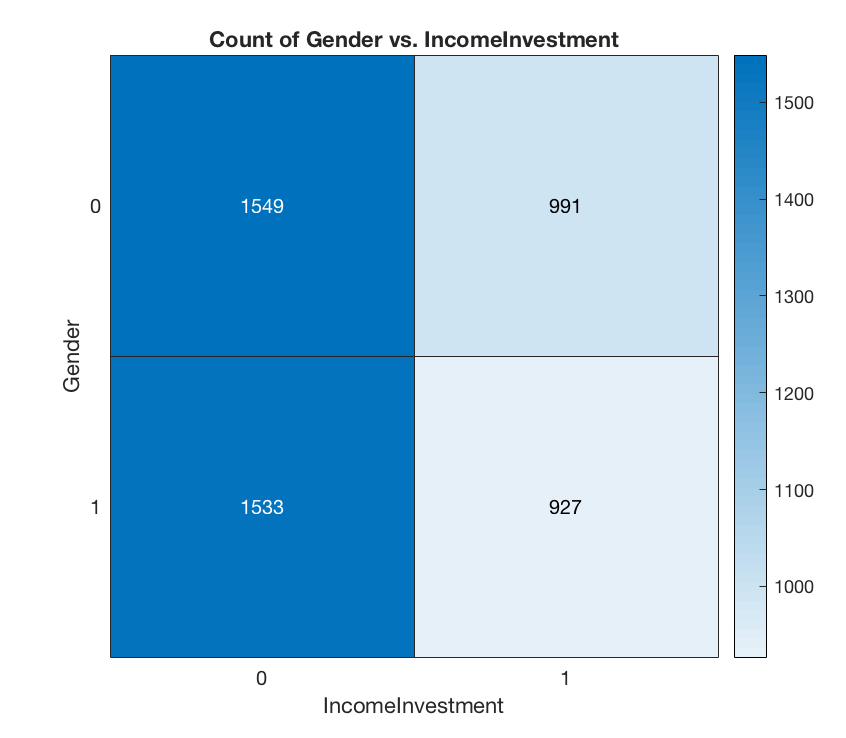
\includegraphics[width=0.48\textwidth]{hm3}
	\end{figure}
\end{frame}

\begin{frame}
\frametitle{Data Transformation}
    \begin{figure}	
		\centering
		\begin{subfigure}[t]{0.48\textwidth}
			\centering
			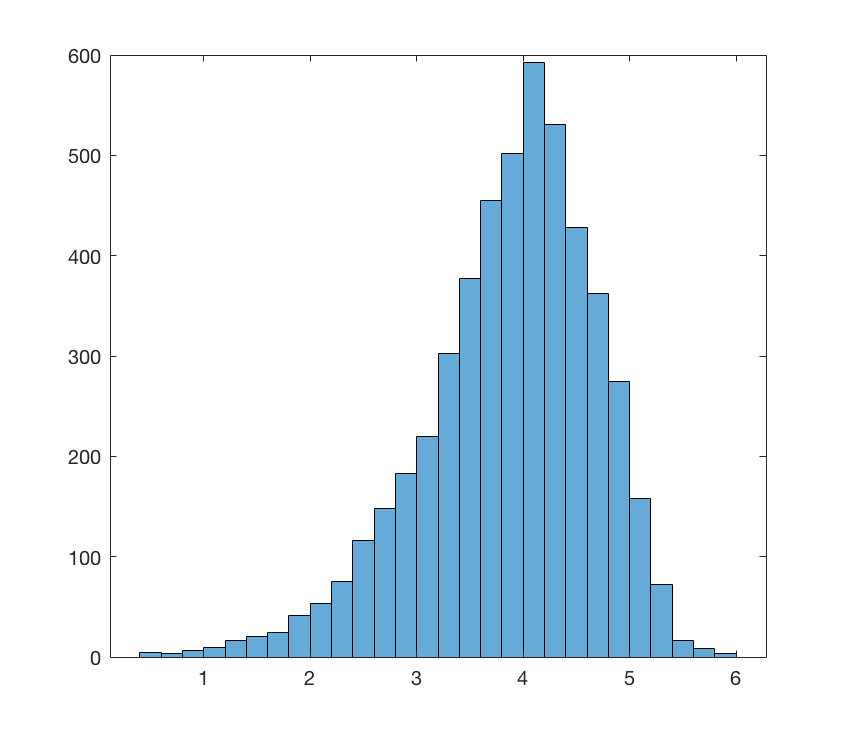
\includegraphics[width=\textwidth]{log_income}
			\caption{$\log$(Income)}
		\end{subfigure}
		\hfill
		\begin{subfigure}[t]{0.48\textwidth}
			\centering
			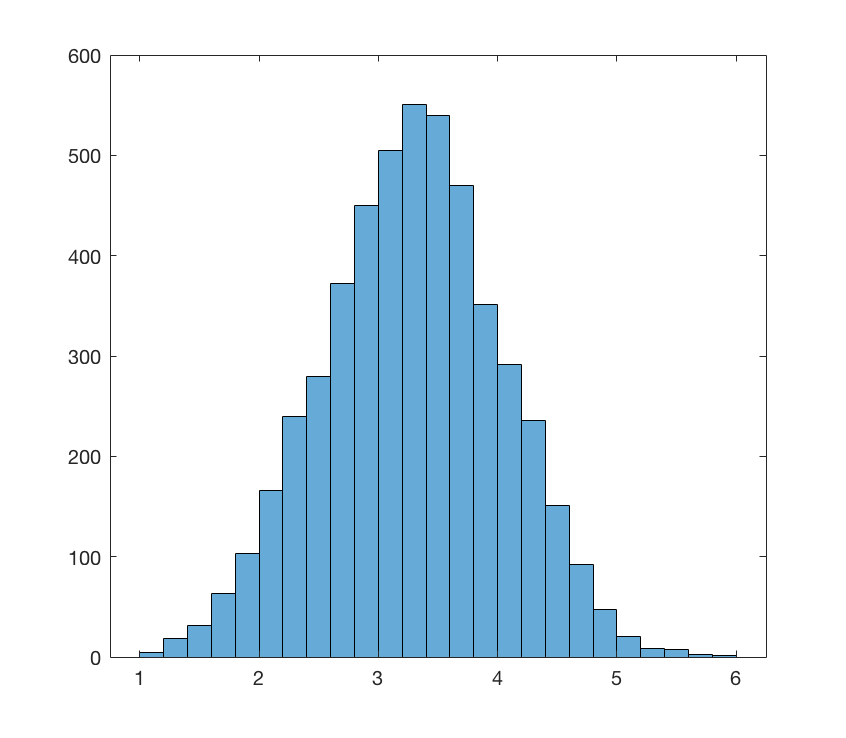
\includegraphics[width=\textwidth]{p03income}
			\caption{Income$^{0.3}$}
		\end{subfigure}
		\caption{Comparison of transformations, we'll go with the second.}
	\end{figure}
\end{frame}


\begin{frame}
\frametitle{Data Transformation}
Using a boxcox transformation, $\text{NewAge} = (\text{OldAge}^{0.9}-1)/0.9.$
\begin{figure}
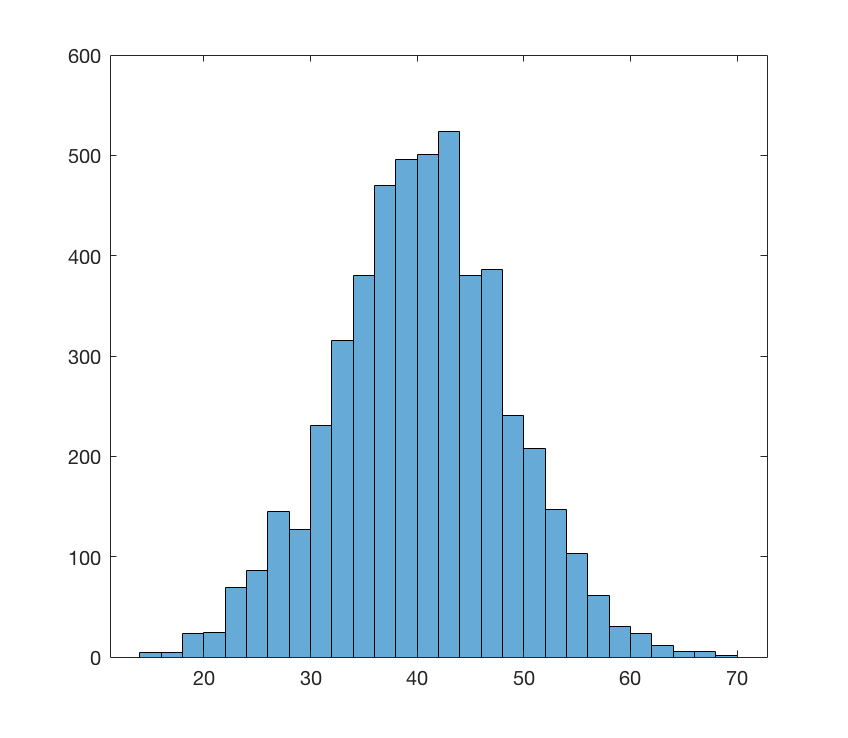
\includegraphics[width=0.6\textwidth]{age_boxcoxed}
\end{figure}
\end{frame}

\begin{frame}
	\frametitle{Data Transformation}
	$\text{NewFinancialEducation} = \text{OldFinancialEducation}^{0.8}$\\
	$\text{NewRiskPropensity} = \text{OldRiskPropensity}^{0.65}$\\
	$\text{NewIncome} = \text{OldIncome}^{0.3}$\\
\end{frame}



\begin{frame}
\frametitle{Cross validation}
	\begin{figure}
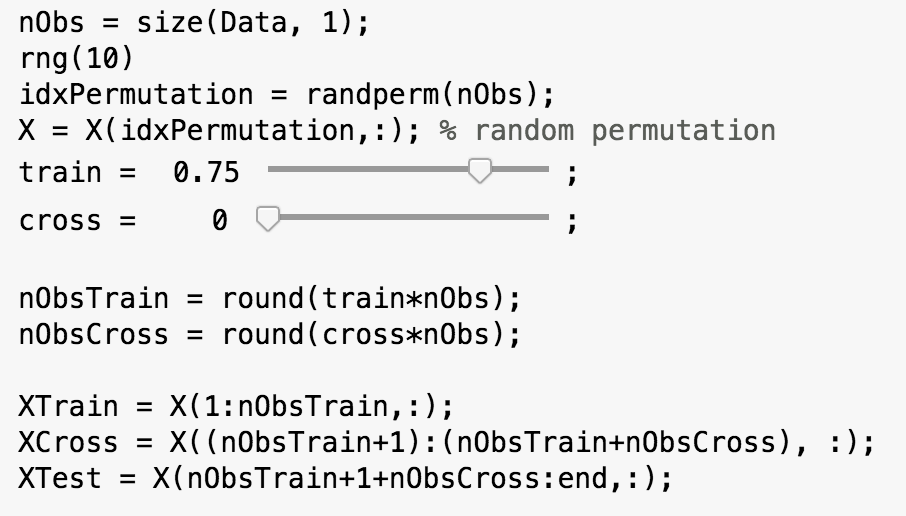
\includegraphics[width=0.6\textwidth]{flex}
\end{figure}
\end{frame}


\begin{frame}[fragile]
\frametitle{Added $Y$ permutation equal to $X$}
\tiny
\begin{verbatim}
YInc = Data.IncomeInvestment;
YInc = YInc(idxPermutation);

yInvIncTrain = YInc(1:nObsTrain);
yInvIncCross = YInc((nObsTrain+1):(nObsTrain+nObsCross));
yInvIncTest = YInc(nObsTrain+nObsCross+1:end);

YAcc = Data.AccumulationInvestment;
YAcc = YAcc(idxPermutation);

yInvAccTrain = YAcc(1:nObsTrain);
yInvAccCross = YAcc((nObsTrain+1):(nObsTrain+nObsCross));
yInvAccTest = YAcc(nObsTrain+nObsCross+1:end);

varNames = {'Age', 'Gender', 'Family', 'FinEdu', 'Risk', 'Income', 'Wealth'};
XTrainTable=table(XTrain(:,1), XTrain(:,2), XTrain(:,3), XTrain(:,4),
XTrain(:,5), XTrain(:,6),XTrain(:,7), 'VariableNames',varNames);
XTestTable=table(XTest(:,1), XTest(:,2), XTest(:,3), XTest(:,4),
XTest(:,5), XTest(:,6),XTest(:,7), 'VariableNames',varNames);
\end{verbatim}
\end{frame}


\begin{frame}
    \frametitle{Classification Learner: model training}
    \begin{figure}
    	\centering
    	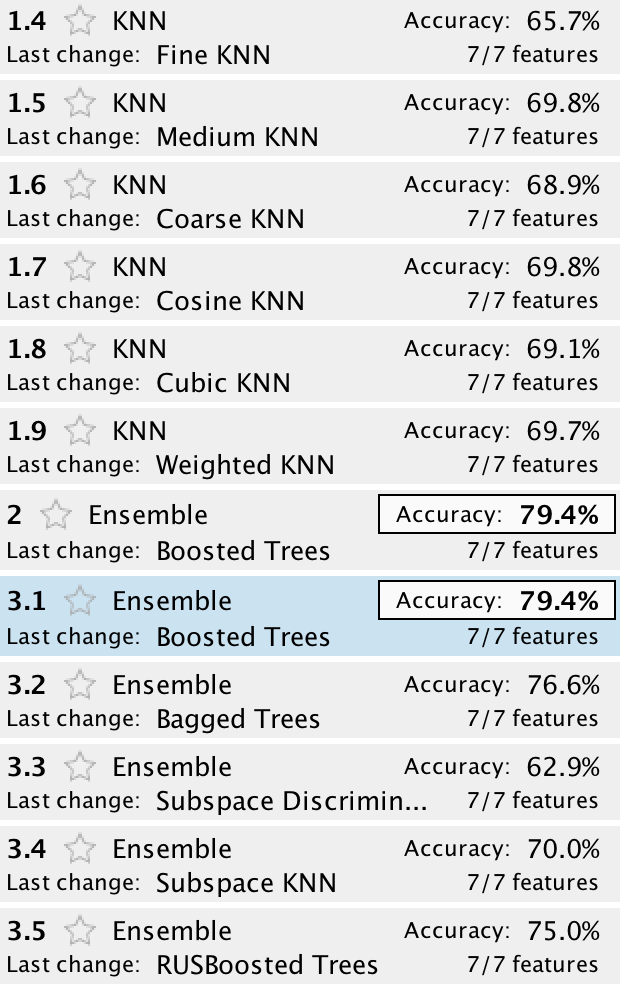
\includegraphics[width=0.35\textwidth]{modelstrained}
    \end{figure}
\end{frame}


\begin{frame}
    \frametitle{Classification Learner: Boosted Tree ROC}
    \begin{figure}
    	\centering
    	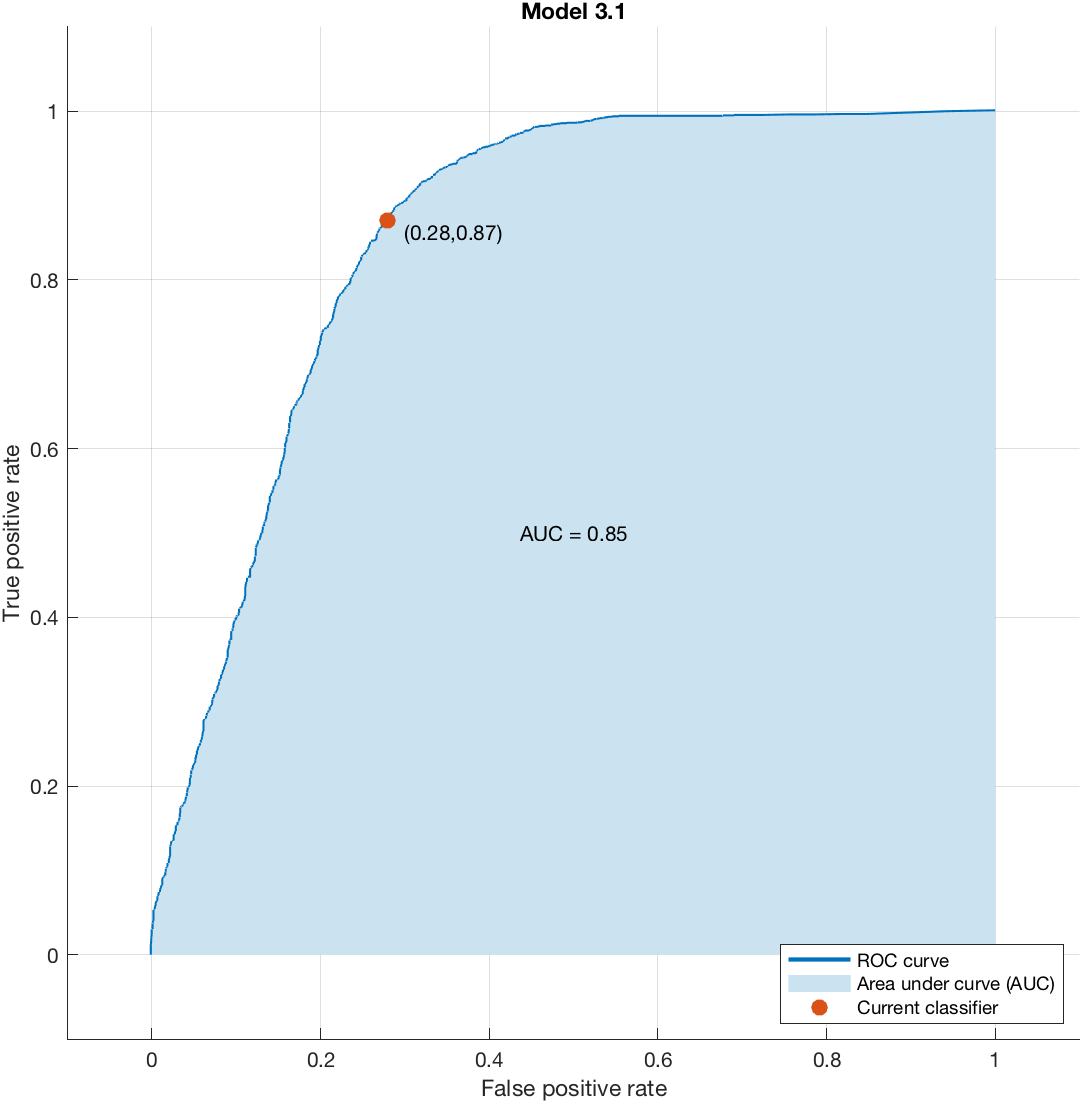
\includegraphics[width=0.6\textwidth]{cl_1_roc}
    \end{figure}
\end{frame}

\begin{frame}
    \frametitle{Classification Learner: Boosted Tree confusion matrix}
    \begin{figure}  
        \centering
        \begin{subfigure}[t]{0.48\textwidth}
            \centering
            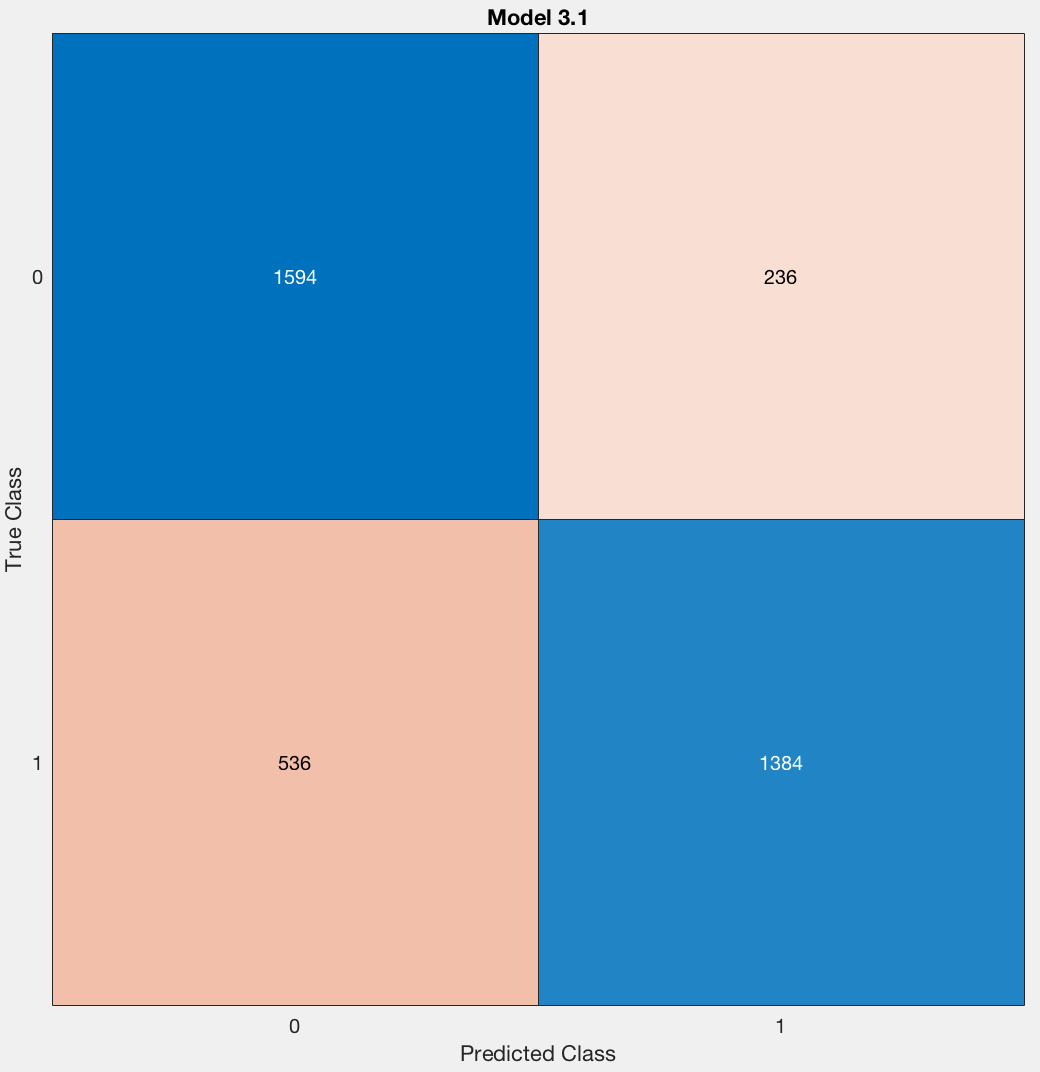
\includegraphics[width=\textwidth]{cl_1_confusion}
            \caption{Confusion matrix.}
        \end{subfigure}
        \hfill
        \begin{subfigure}[t]{0.48\textwidth}
            \centering
            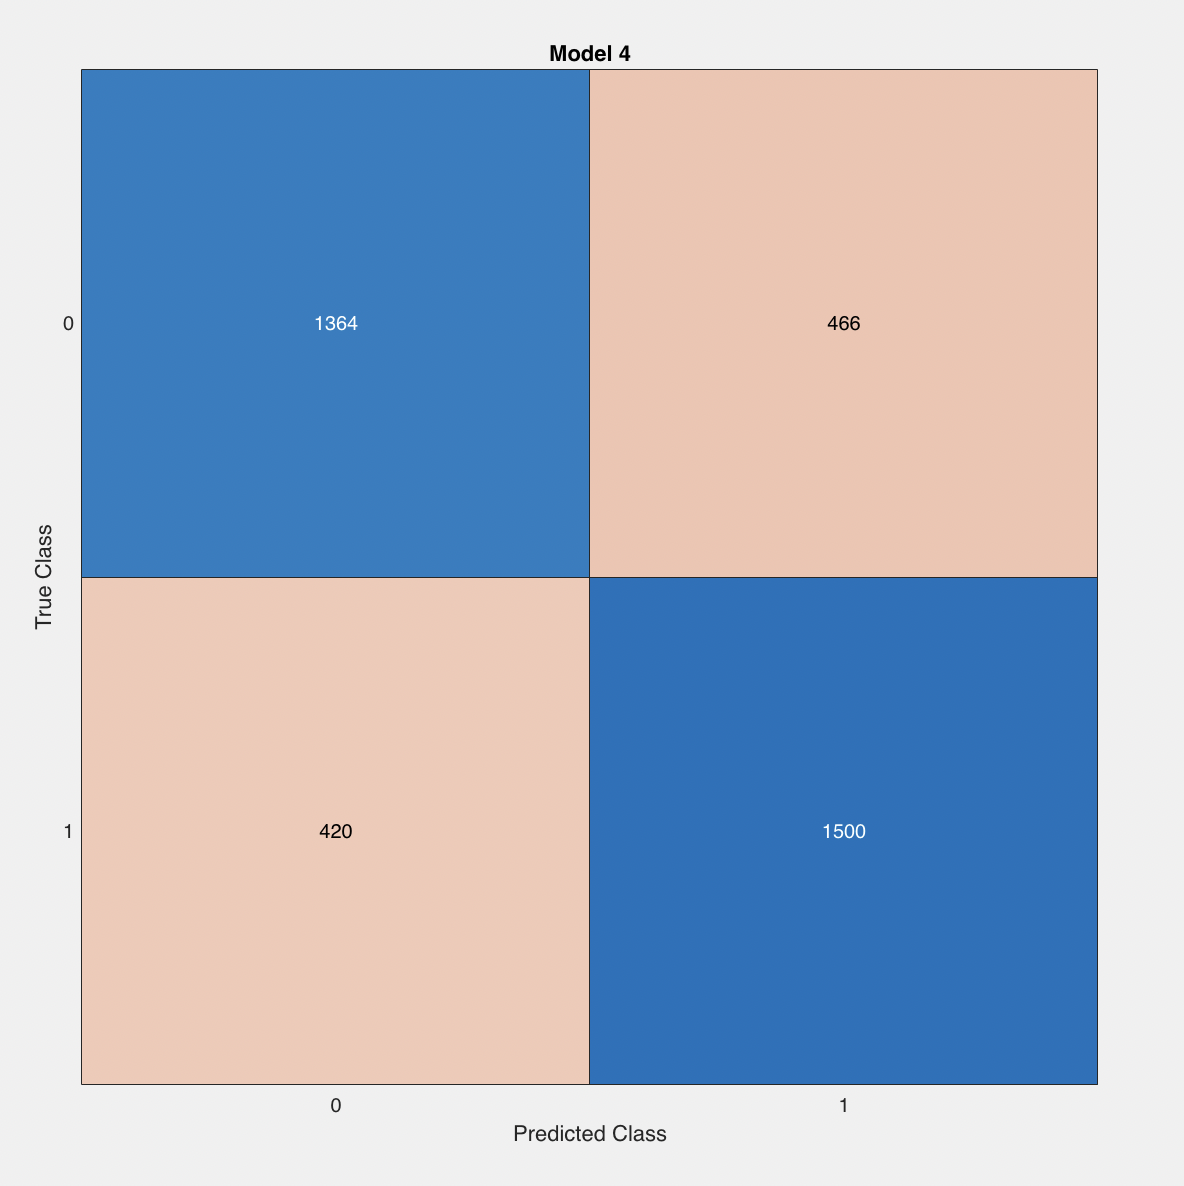
\includegraphics[width=\textwidth]{cl_1_confusion_penalized}
            \caption{Penalized confusion matrix.}
        \end{subfigure}
        %\caption{Comparison of transformations, we'll go with the second.}
    \end{figure}
\end{frame}

\begin{frame}[fragile]
\frametitle{Reducing data}
We remove \texttt{Gender} and \texttt{FamilySize}
\tiny
\begin{verbatim}
Xsmall = [rescale(IncomeWealthRatio) rescale(pAge) rescale(pFin) rescale(pIncome) rescale(pWealth)];
Xsmall = Xsmall(idxPermutation,:);
XsmallTrain = Xsmall(1:nObsTrain,:);
XsmallTest = Xsmall(nObsTrain+1:end,:);
XsmallTrainTable=table(XsmallTrain(:,1), XsmallTrain(:,2), XsmallTrain(:,3),
XsmallTrain(:,4), XsmallTrain(:,5), 'VariableNames',xnames);
\end{verbatim}
\end{frame}

\begin{frame}
    \frametitle{Classification Learner: model training}
    \begin{figure}
    	\centering
    	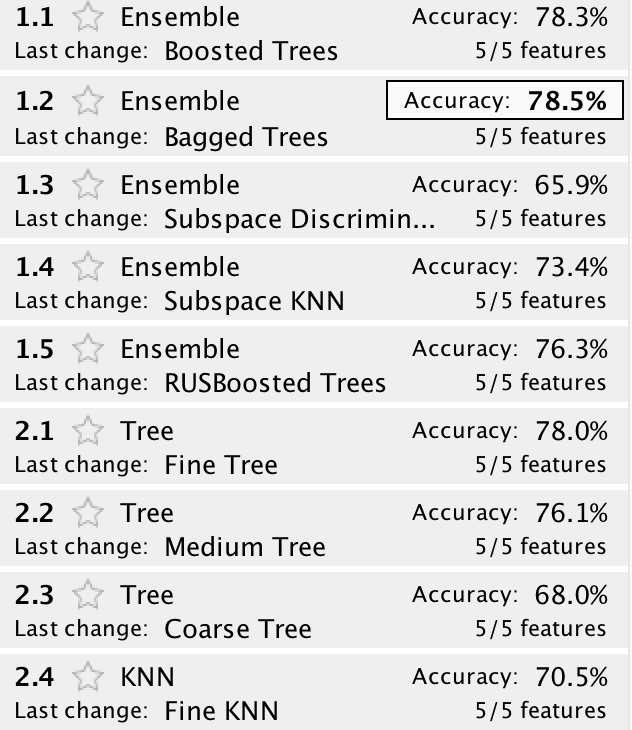
\includegraphics[width=0.35\textwidth]{modelstrained_small}
    \end{figure}
\end{frame}

\begin{frame}
    \frametitle{Classification Learner: Bagged Tree ROC}
    \begin{figure}
    	\centering
    	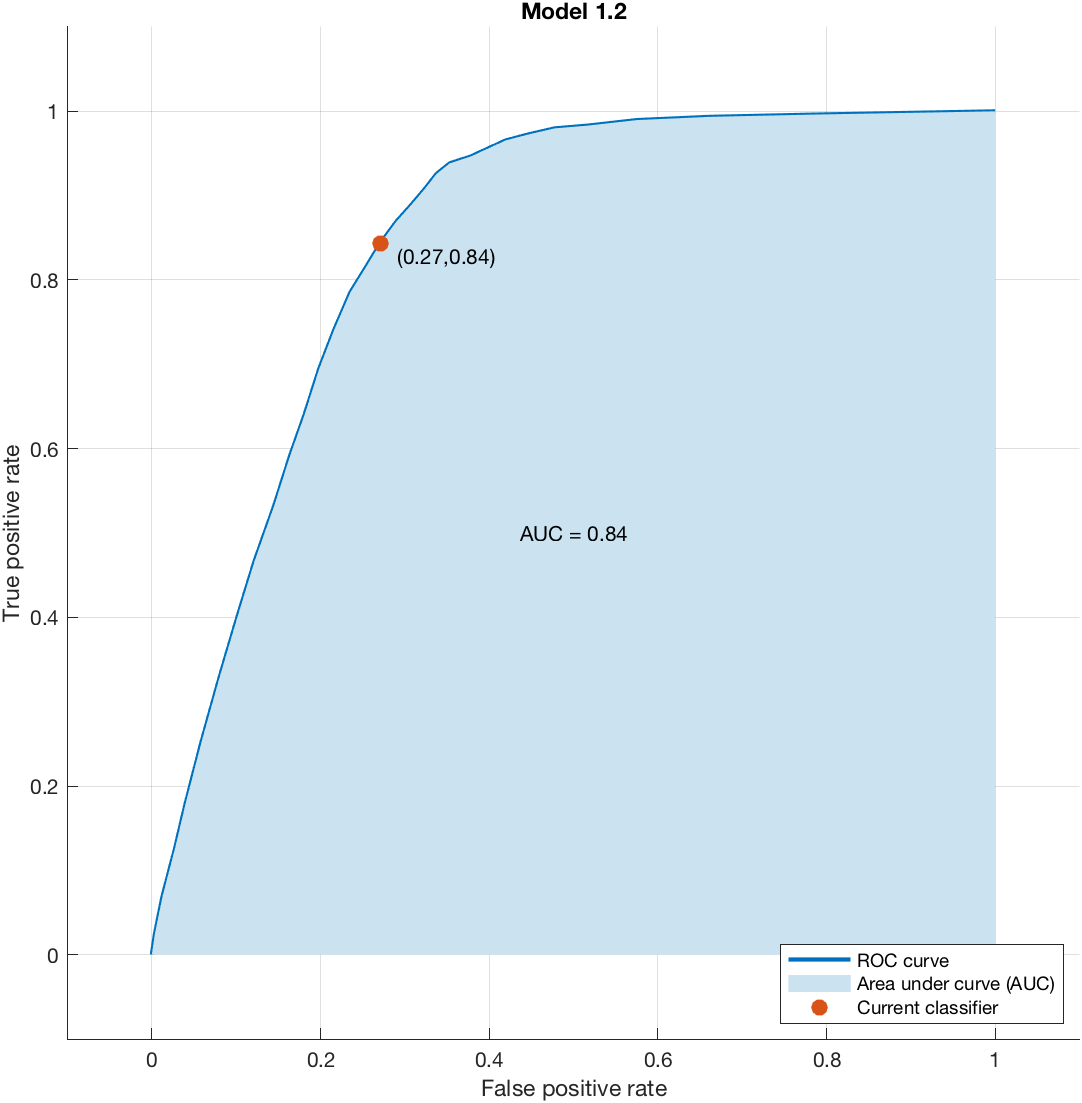
\includegraphics[width=0.6\textwidth]{cl_2_roc}
    \end{figure}
\end{frame}

% \begin{frame}
%     \frametitle{Classification Learner: Bagged Tree confusion matrix}
%     \begin{figure}
%     	\centering
%     	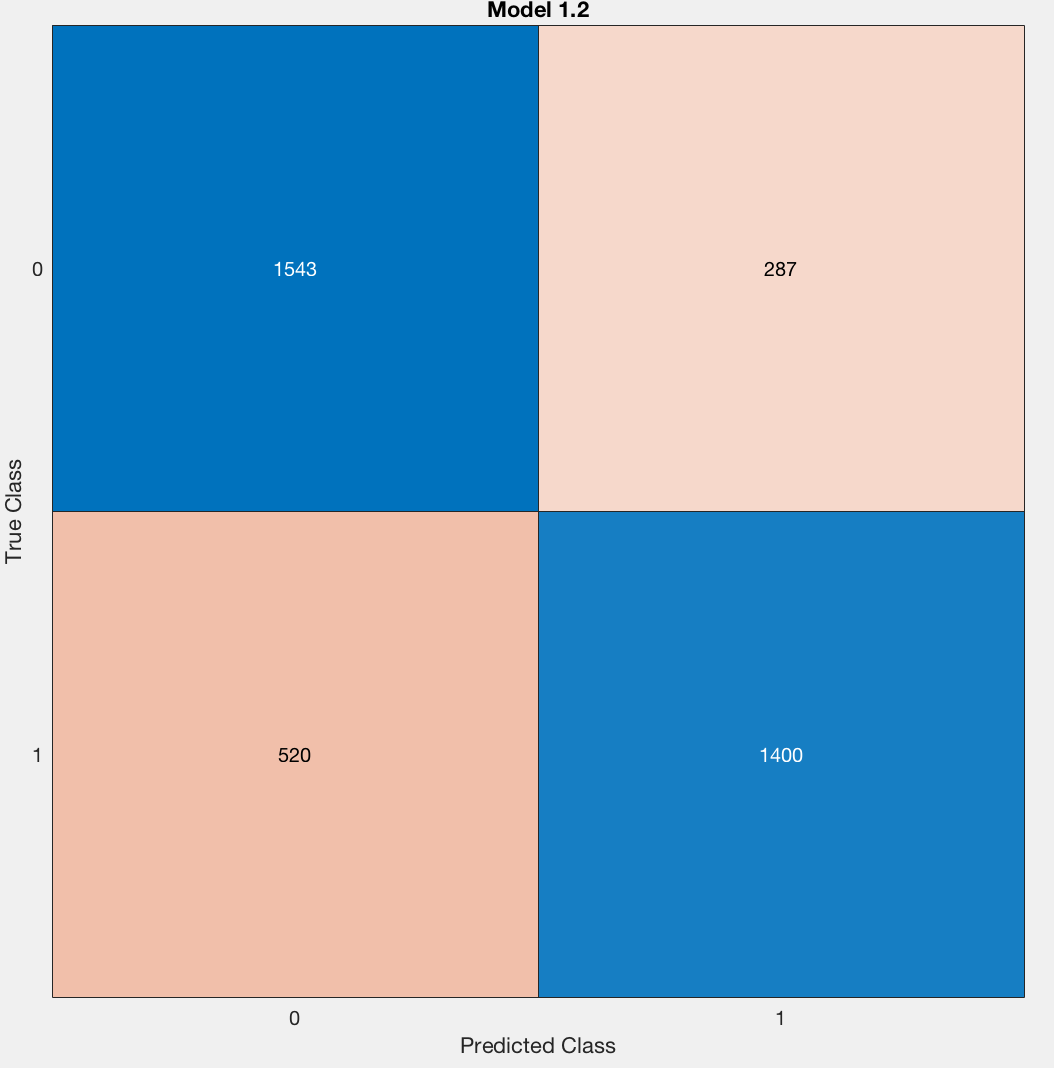
\includegraphics[width=0.6\textwidth]{cl_2_confusion}
%     \end{figure}
% \end{frame}

\section{Recommending products}

\begin{frame}
\frametitle{Recommending products}
Using Bayesian optimization we decide to use the Bagged Tree model after evaluating 30 alternatives.
\end{frame}

\begin{frame}
    \frametitle{Product recommendation based on Risk Propensity}
    \begin{figure}
    	\centering
    	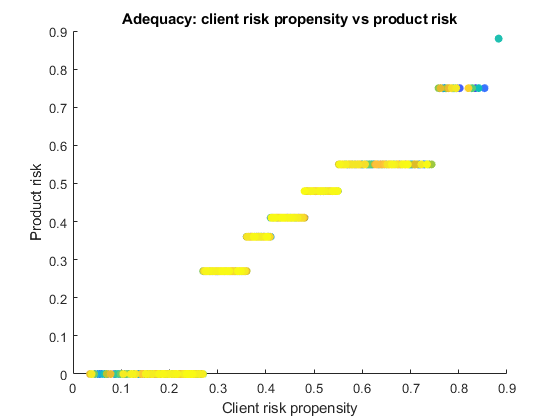
\includegraphics[width=0.6\textwidth]{recomm1}
    \end{figure}
\end{frame}

\section{Further development points}

\begin{frame}
    \begin{itemize}
        \item more data cleaning to improve model accuracy;
        \item better data visualization for product recommendation.
    \end{itemize}
\end{frame}







\end{document}